\documentclass{article} % Defines the document class, article is commonly used
\usepackage[shortlabels]{enumitem}
\usepackage{amsmath}    % Allows for more advanced math formatting
\usepackage{amssymb}    % Provides additional mathematical symbols
\usepackage{amsthm}     % \qed
\usepackage{graphicx}   % image
\usepackage{float}      % image placement
\usepackage{siunitx}
\usepackage{hyperref}
\hypersetup{
    colorlinks=true,       % false: boxed links; true: colored links
    linkcolor=black,       % color of internal links
}
\usepackage[margin=1.5in]{geometry}

\begin{document}

\title{EEC133 Pre-Lab 2: Loop Antennas}
\author{Tao Wang}
\date{\today}

\maketitle
\tableofcontents

\section*{Pre-Lab}
\addcontentsline{toc}{section}{Pre-Lab}

\subsection*{Part 1: Loop Antenna Design}
\addcontentsline{toc}{subsection}{Loop Antenna Design}

\subsubsection*{Questions:}
\begin{enumerate}
    \item $r = 0.0064 \si{m}$. $\lambda = \frac{c}{f} = 0.12 \si{m}$. $r \leq \frac{\lambda}{6 \pi} \approx 0.00637 \si{m}$.
    \item
          \[\text{Radiation Resistance: }320 \pi^6 \left(\frac{0.00637}{0.12}\right)^4 = 2.44 \Omega \]
          \[\text{Directivity: } 1.5\]
          \[\text{Half-power beamwidth: } \frac{\pi}{2}\]
          \[\text{Far Field Requirement: } r >> \frac{0.12}{2\pi} = 0.019 \si{m}\]
    \item
          \begin{figure}[H]
              \centering
              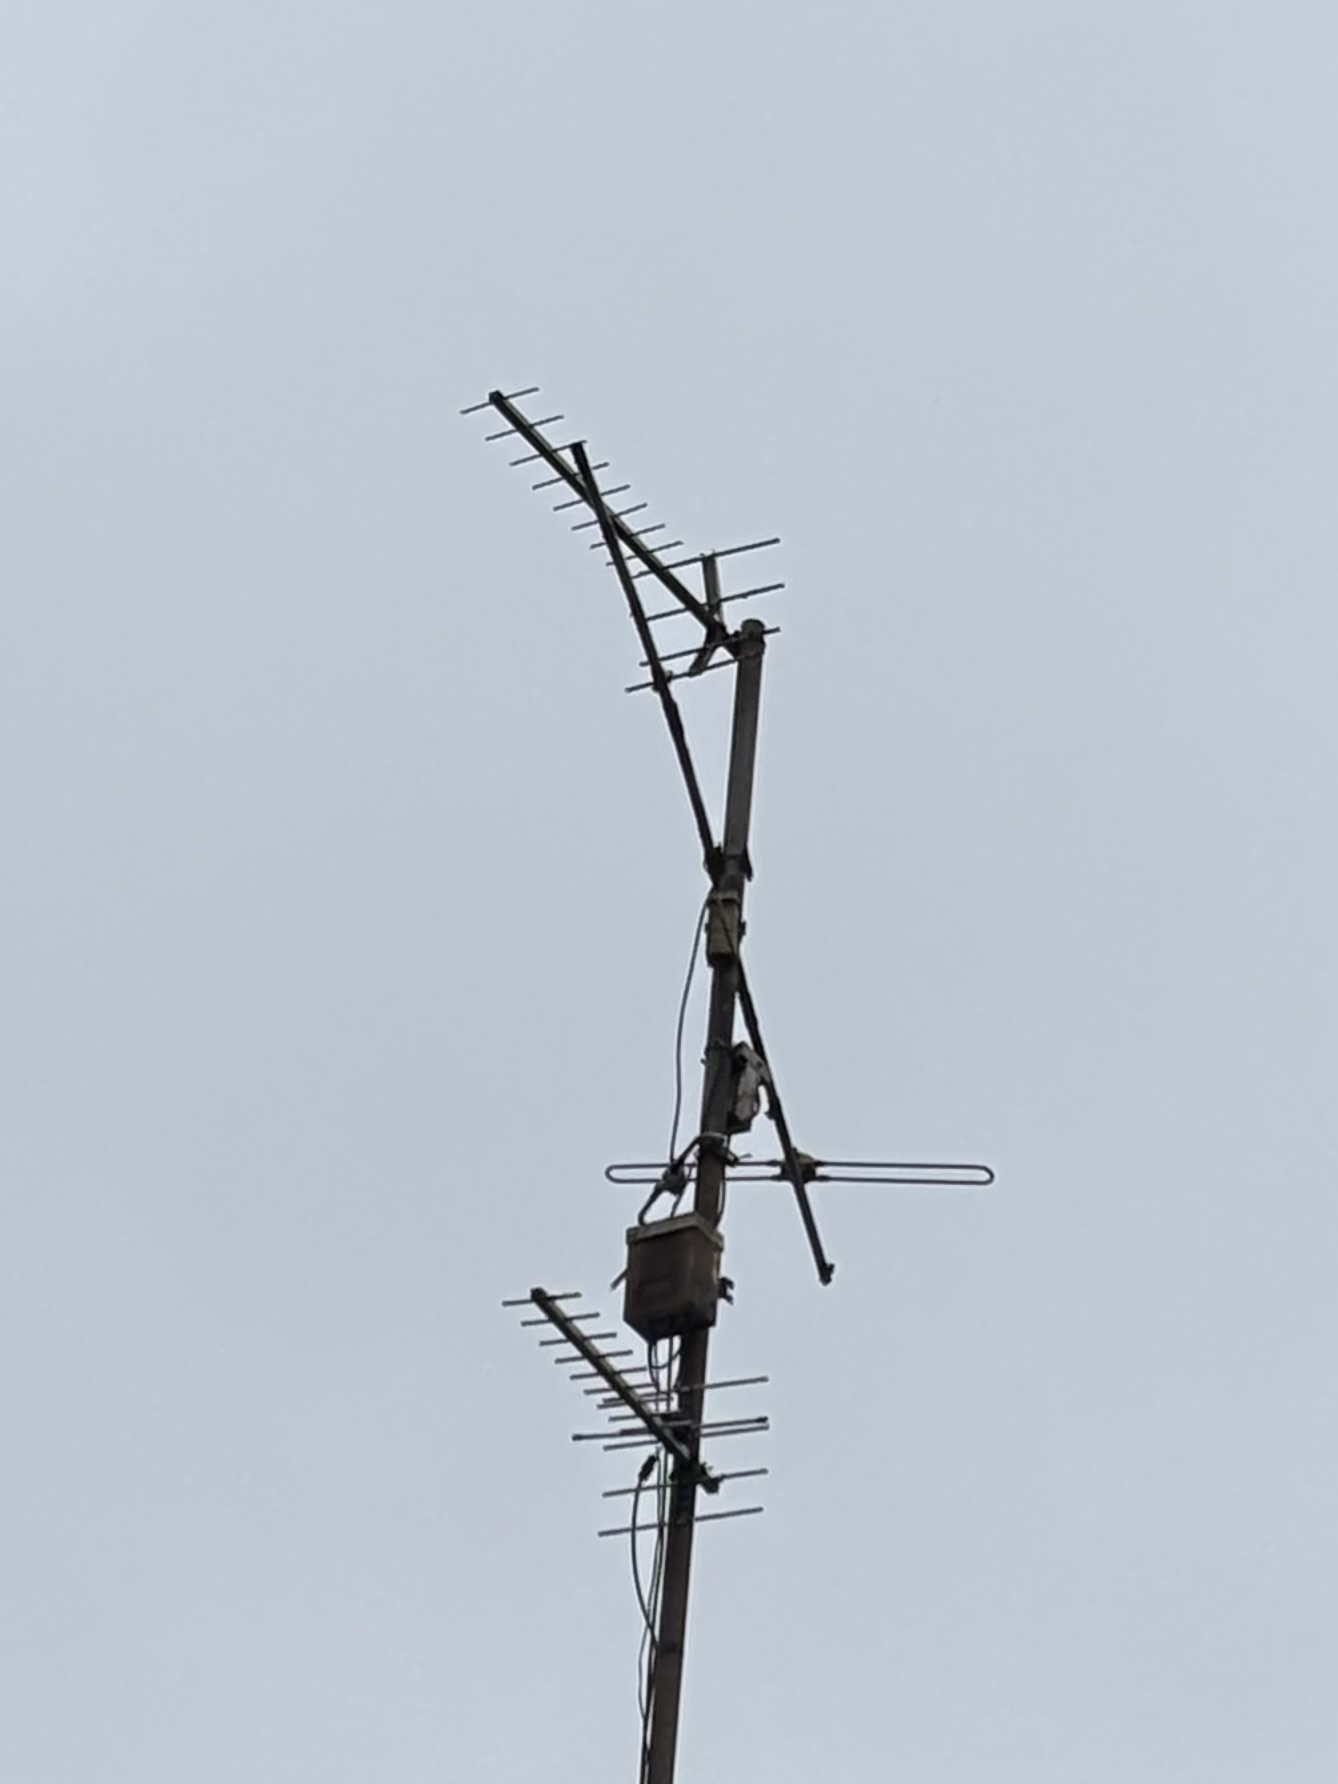
\includegraphics[width=1\textwidth]{./image/figure1.png}
              \caption{}
          \end{figure}
\end{enumerate}

\section*{Part 2: More Noise Calculations}
\addcontentsline{toc}{section}{Part 1: More Noise Calculations}

\subsection*{Questions:}
\begin{enumerate}
    \item $R_{in}$ and $R_{out}$ are typically $50 \Omega$ to avoid wave reflection in $R_{in}$ by matching the characteristics impedance in the input and output transmission line. $R_{out}$
    \item Noise =
          \[9.1*10^{-10} \frac{V}{\sqrt{Hz}}\]
          This unit means that the noise voltage is $9.1*10^{-10}$ volts per unit of the frequency bandwidth.
    \item $R_{in} = 0.489 \Omega$, so $\tau = 0.019$. The small transmission coefficient implies that very little power will be transmitted to the amplifier, so the signal amplification will be poor.
\end{enumerate}



\end{document}
